\normalfont\normalsize
\chapter{Hardware Platform}

In this chapter we will present the hardware platforms used in the development of the algorithm. The variety of platforms was
a key point in designing the scenario to test the algorithm, as this demonstrates that task modelling of application abstractizes
beyond platforms, making heterogenous wireless sensor networks such as these possible.

We will discuss the platforms in chronological order of use, our WSN started off with the Raven development kits. The next step
was for our team to develop our own wireless sensor nodes based upon wireless modules (the Zigbit module), and these are the 
Sparrow nodes. The Power Sparrow nodes inherit much of the original, but have very specific purpose, measuring power usage of 
appliances.

All platforms run the Contiki Operating System and will have the same core of software functionalities. Additional capabilities will be given
by the presence of sensors attached to the platforms.  Other differences will be in measuring the power used by system, measured by the
system itself. There will be inherent differences as to how this is handled on each platform, mainly because of the hardware design and
technology used, as well as expansion connectors provided.

The heterogeneity of the platforms must not be seen as similar ways to do the same thing, each platform best suits a specific purpose.
The Raven nodes are an all-in-one sensor boards, with user interface, Sparrow nodes have an expansion board for energy harvesting 
experiments, Power Sparrow measure outlet voltage, powering themselves directly from the outlet.

\clearpage

\section{The AVR Raven development kit}



The AVR Raven developed by Atmel is a development kit for the AT86RF230 radio transceiver. A kit usually consists of two AVR Raven
wireless nodes and one Raven USB stick that acts as a gateway. The stick is connected to a PC (or embedded system) and acts as a 
remote wireless card, offering an additional interface to communicate with the nodes.

\begin{figure}[ht]
\begin{center}
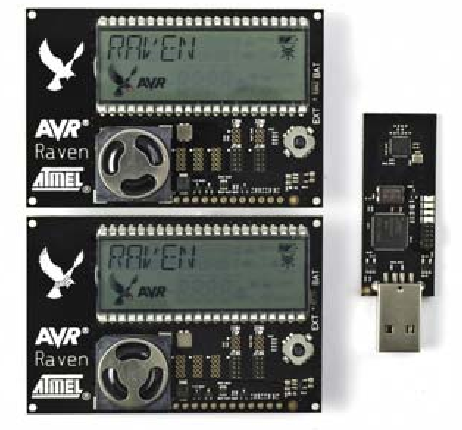
\includegraphics[scale=0.5]{hw_platform/raven.png}
\end{center}
\caption{\small \itshape{The AVR Raven development kit}}
\end{figure}

This forms a versatile kit that can be used for debugging or building a variety of RF applications in the 802.15.4 frequency range:
from point-to-point communication to large WSNs(using more than one kit). Using more than one Raven USB Stick, even multi-sink networks 
can be formed, apart from the usual single-sink networks that can be built with only one kit.

\subsection{The Raven Nodes}

Individual Raven Nodes are built around two microcontrollers, the Atmega1284P and the Atmega3290P, the former dealing with radio communication 
and the latter with the user interface peripherals. These microcontrollers are selected from the picoPower family, ensuring minimal power consumption
and viable operation down to low supply voltages (1.8V). The Raven Node communicates wirelessly via a transceiver chip (the AT86RF230) and has a 
built-in PCB antenna.

\begin{figure}[ht]
\begin{center}
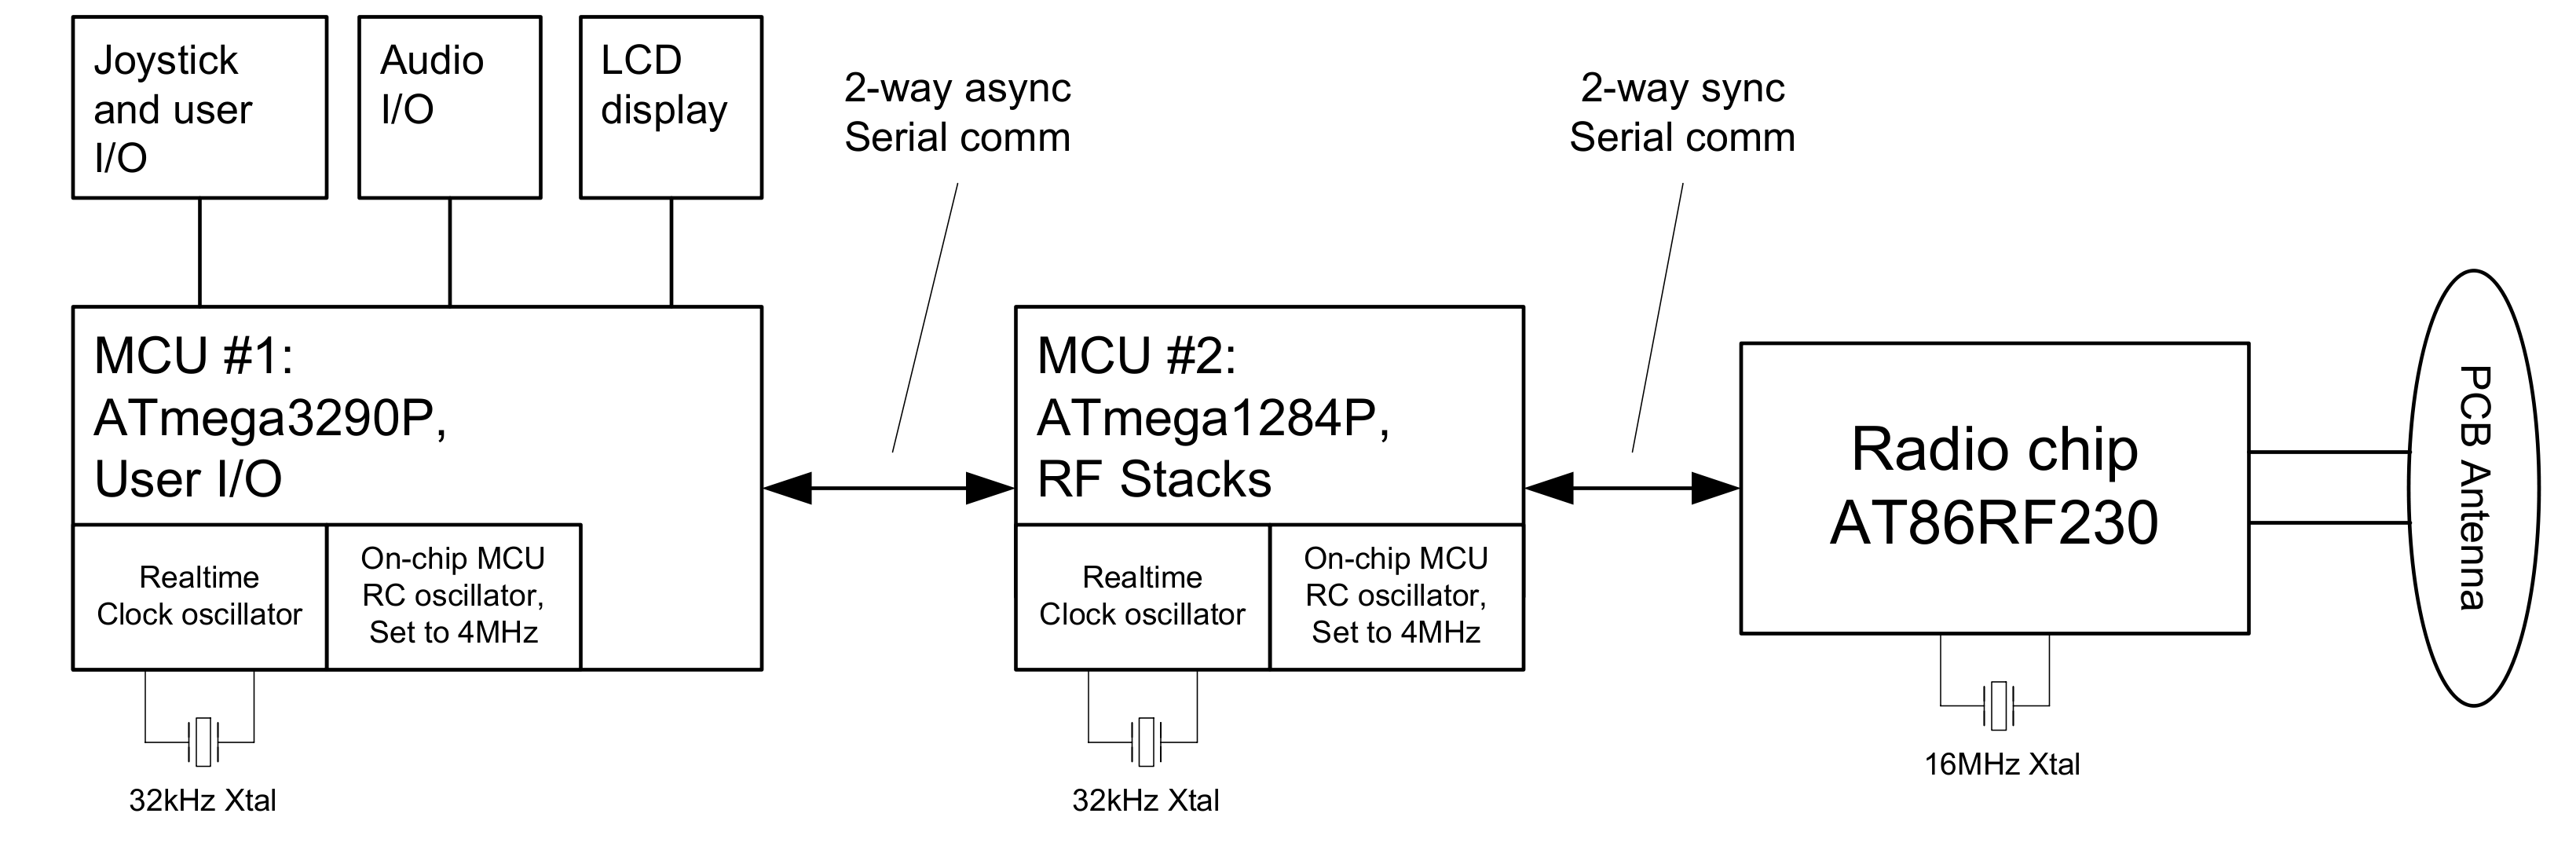
\includegraphics[scale=0.9]{hw_platform/raven_node_overview.png}
\end{center}
\caption{\small \textit{Overview of an AVR Raven node}}
\end{figure}


Communication between the two microprocessors and between the Atmega128 and the radio transceiver is accomplished through a synchronous serial
interface (\textbf{USART} - Universal Synchronous Asynchronous Receiver Transmitter).

The Atmega1284P holds the wireless stack code and acts upon user input on the other microcontroller. It uses a  32.768 kHz oscillator for a realtime
clock, but its main clock is internal, set at 4MHz.

The Atmega3290P drives the Raven LCD, has audio output/input and a joystick as human interface. It also maintains a 32.768 kHz oscillator for realtime 
clock purposes besides its main clock of 4MHz. Audio output on the node is controlled with PWM, whose signal passes through a low-pass filter and a 
class-D amplifier before reaching the 8$\Omega$ speaker. A microphone is connected to the node for audio output, the signal is amplified and low-pass 
filtered before reaching one of the ADC (Analog-to-Digital Converter) pins on the chip.  

Each microcontroller has a chip with persistent memory attached, the Atmega1284P has a 2Kbits Serial EEPROM (AT24C02B) attached on TWI (Two-Wire
Interface). This memory holds configuration and calibration data that are write-protected. The Atmega3290P has a 16MBits Serial Dataflash attached. 
This memory is designed to hold firmware images as well as sounds. It will operate however only when the supply voltage is above 2.5V, unlike the rest
of the system (If batteries are low the Raven node might still be able to transmit but it will not be able to read/write data from the external dataflash.

The PCB antenna is a folded dipole antenna of $100\Omega$ with a net peak gain of 5dB.

The power supply for the node can be internal (LR44 batteries), or external, with supply voltages ranging from 5V to 12V. The external supply voltage
also passes through a voltage divider and is connected to 2nd ADC pin of the Atmega3290P microcontroller, therefore the node can monitor the external
operating voltage.

The Raven node exposes both JTAG and ISP programming connectors, together with several GPIO headers.

\subsection{The Raven USB Stick}


\begin{figure}[ht]
\begin{center}
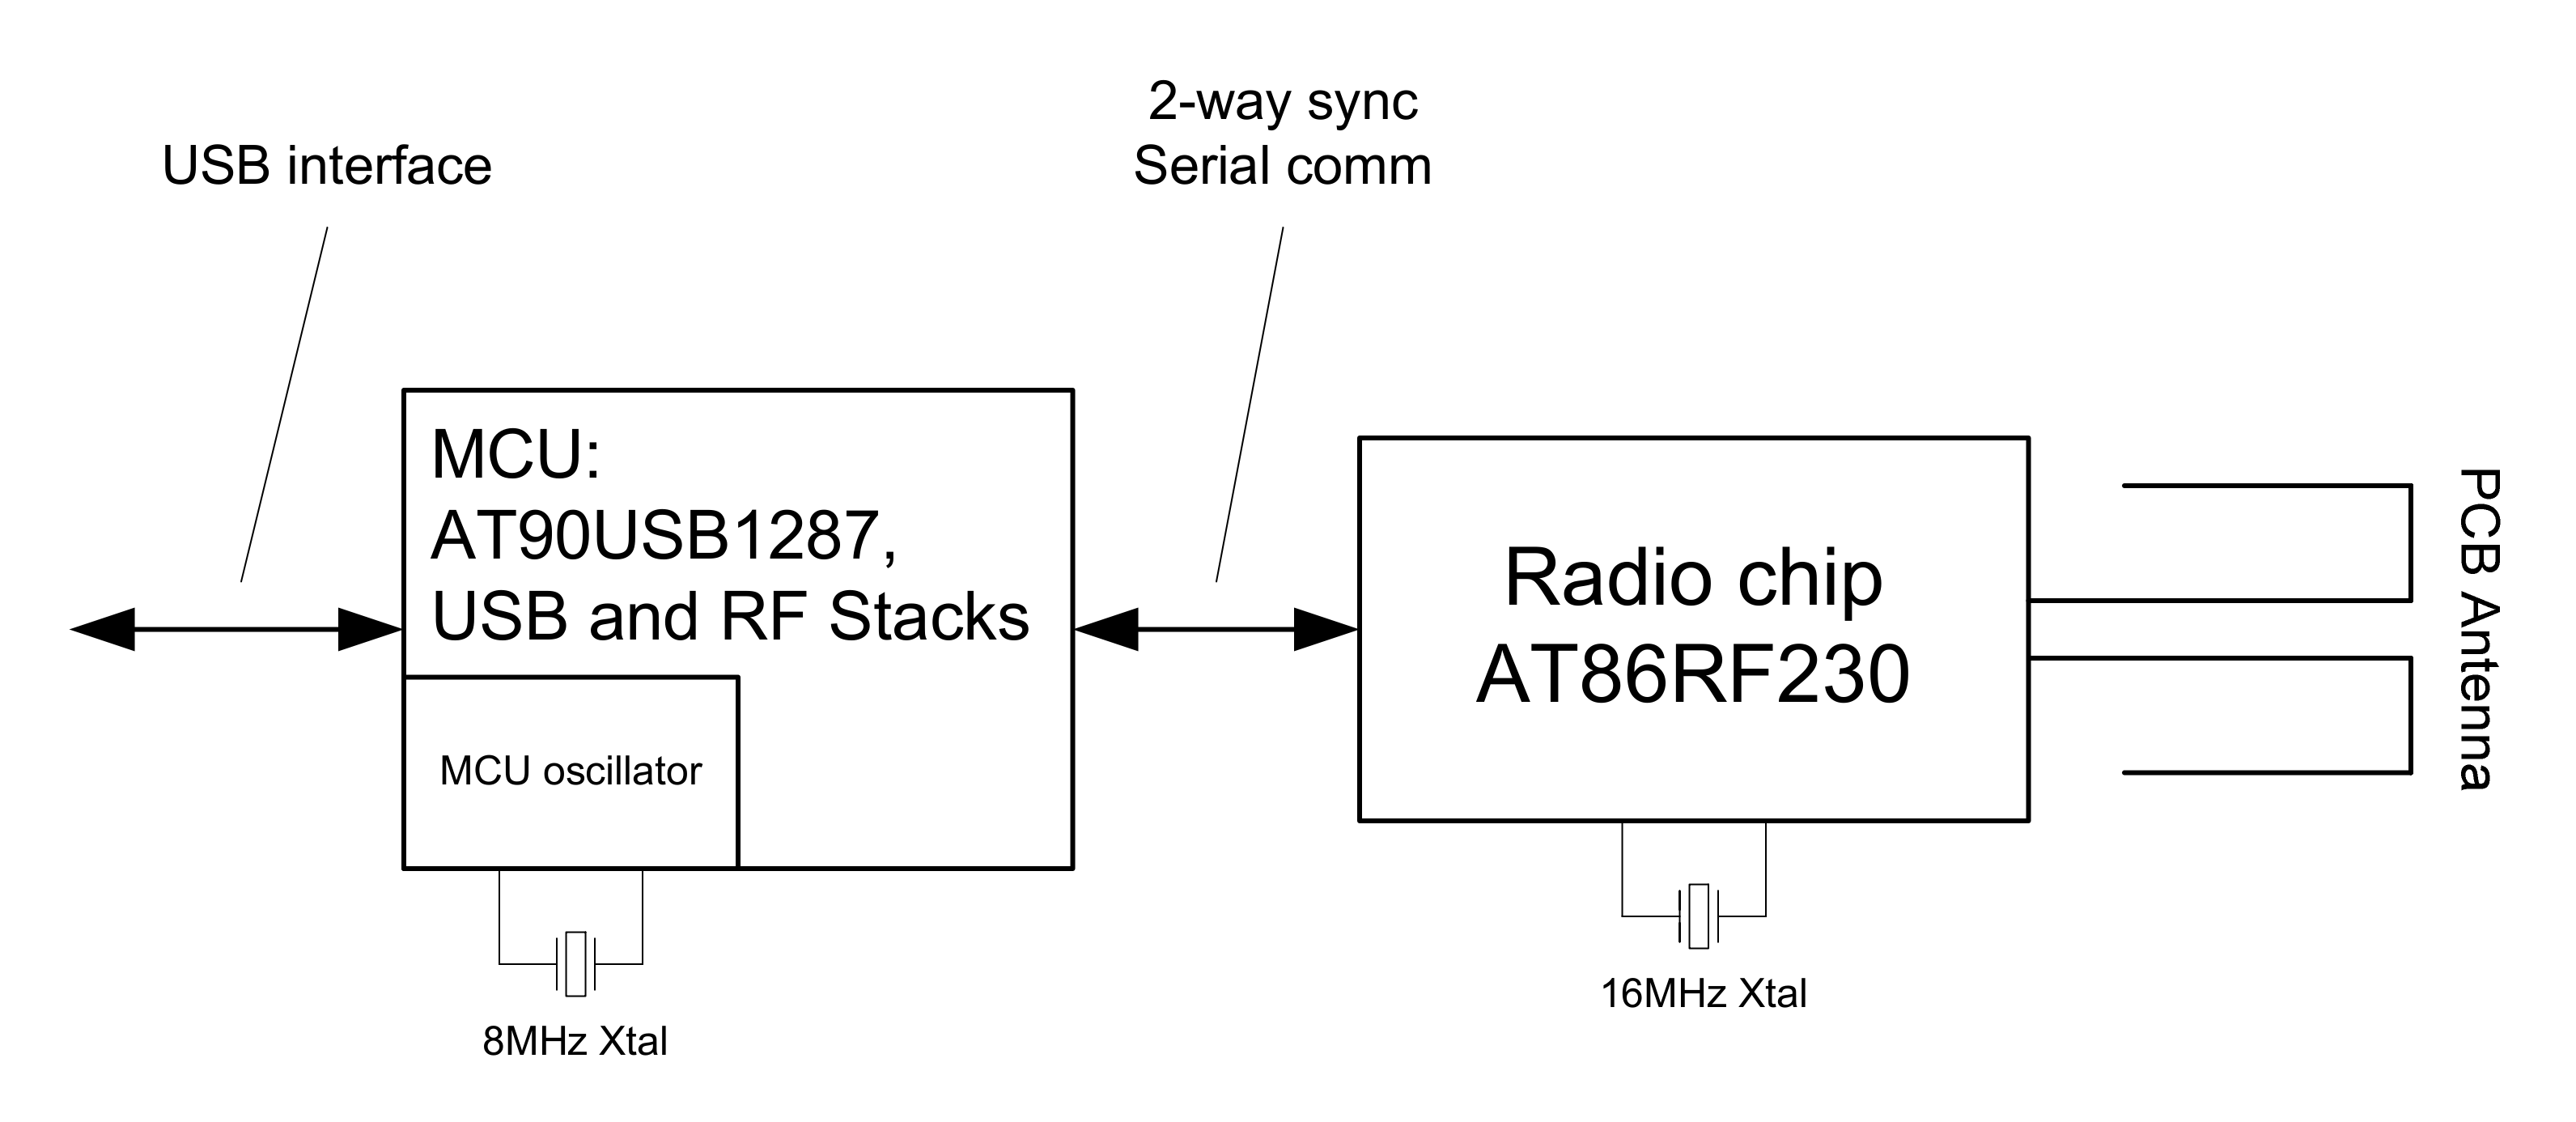
\includegraphics[]{hw_platform/raven_stick_overview.png}
\end{center}
\caption{\small \itshape{Overview of an AVR Raven USB Stick}}
\end{figure}
The Raven USB Stick is built around a USB-capable microcontroller and the same AT86RF230 radio transceiver chip. The USB-capable 
microcontroller is the AT90USB1287, capable of acting as a full speed USB device. With the Contiki Operating System, the USB Stick
acts as a gateway for the WSN and as a remote network interface (RNDIS) on the computer it is connected to.

The antenna on the Raven USB stick is a dipole antenna with a net peak gain of 0 dB.

It has a JTAG programming interface and a serial interface for ``printf`` debugging, along with 4 LEDs to show current status.


\section{Sparrow Wireless Sensor} 

\begin{figure}[ht]
\begin{center}
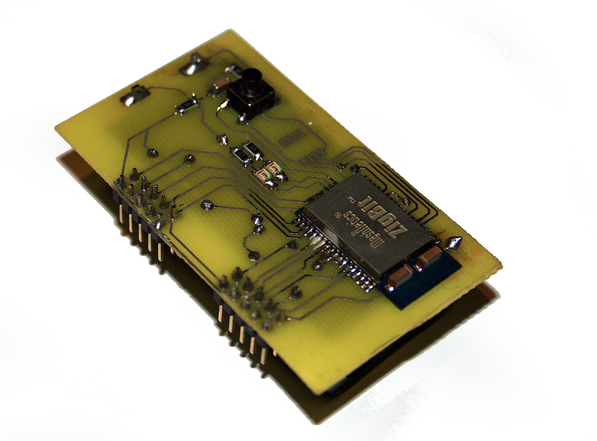
\includegraphics[scale=0.5]{hw_platform/sparrow.png}
\end{center}
\caption{\small \itshape{The Sparrow wireless node}}
\end{figure}
The sparrow is a sensor node built around the powerful Zigbit\texttrademark module. It provides a JTAG header for programming,
and expansion connectors for two USARTs (Universal Synchronous/ Asynchronous Receiver Transmitter), one TWI (Two-Wire Interface)
and 3 ADC channels (Analog-to-Digital Converter).



For user interaction there is a switch and a couple of leds. As sensing capabilities, it has a SHT11 humidity and temperature
sensor connected by a software SPI (Serial Peripheral Interface).

\subsection{Zigbit\texttrademark    module}

The Zigbit\texttrademark   module is an all-in-one wireless module, consisting of an Atmega128 microcontroller, a RF 
transceiver chip and a dual chip antenna, being perfect for small-footprint wireless sensor applications. It is designed 
to operate in the 2.4GHz band, as a 802.15.4/Zigbee node. Its high sensitivity and low-power guarantee fitness for any 
wireless application.

The mixed-signal small-footprint package make it ideal for rapid prototyping and research endeavours.
\begin{figure}[ht]
\begin{center}
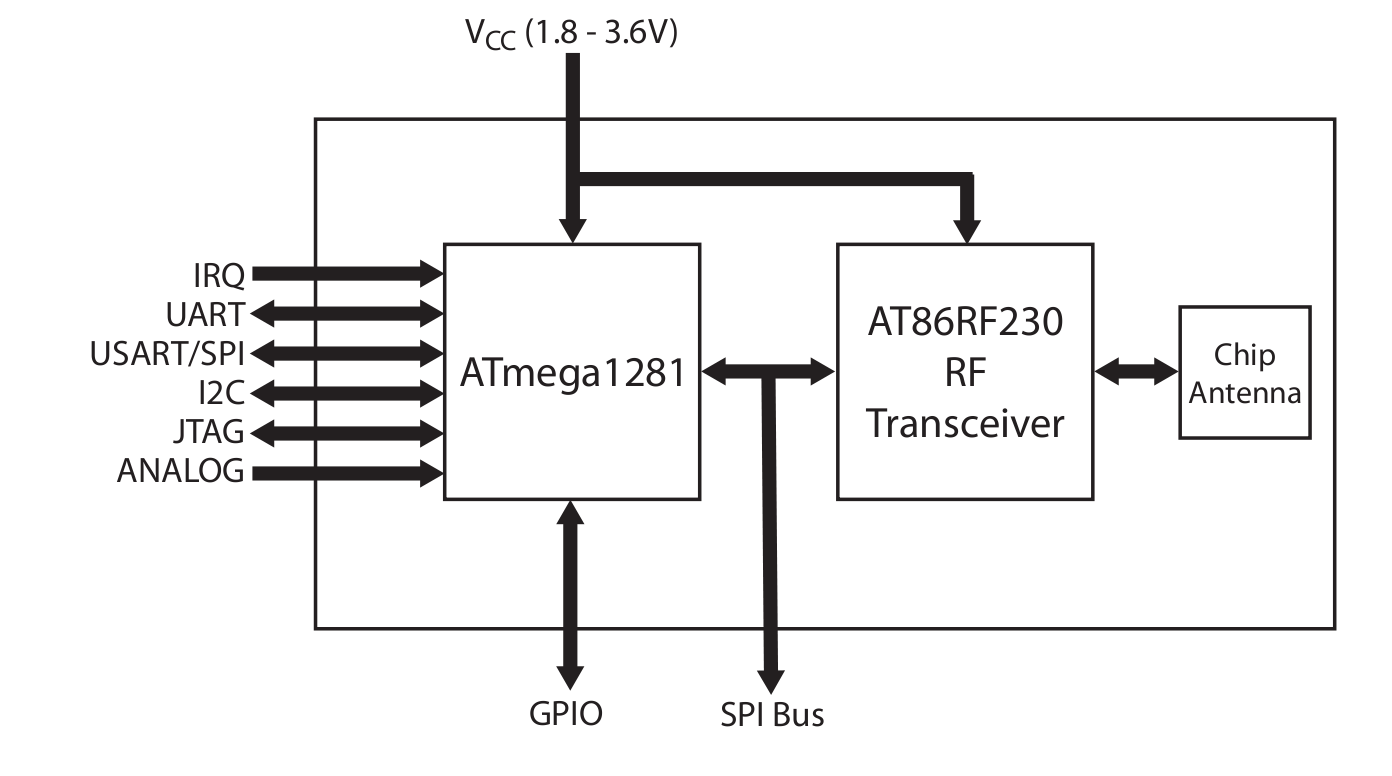
\includegraphics{hw_platform/zigbit.png}
\end{center}
\caption{\small \itshape{Overview of the Zigbit\texttrademark   module architecture}}
\end{figure}

\section{Sparrow Power}

The Power version of the Sparrow nodes are built so that they can obtain their power directly from the power outlet they will 
measure. The wireless part still uses the Zigbit\texttrademark module,but additional circuitry has been added to be able to 
sample voltage and current at the outlet.

\begin{figure}[ht]
\begin{center}
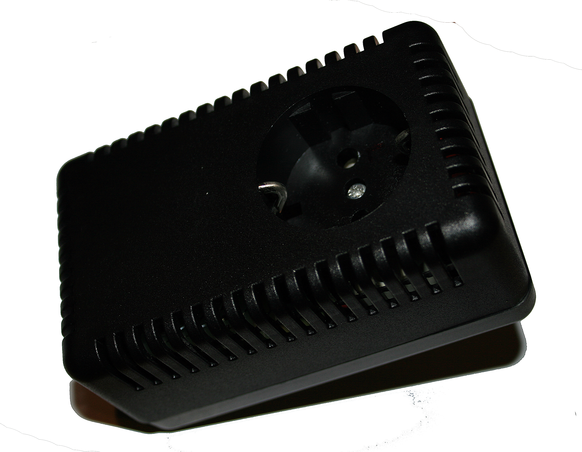
\includegraphics[scale=0.5]{hw_platform/sparrowpower1.png}
\end{center}
\caption{\small \itshape{The Sparrow Power wireless device}}
\end{figure}


\begin{figure}[ht]
\begin{center}
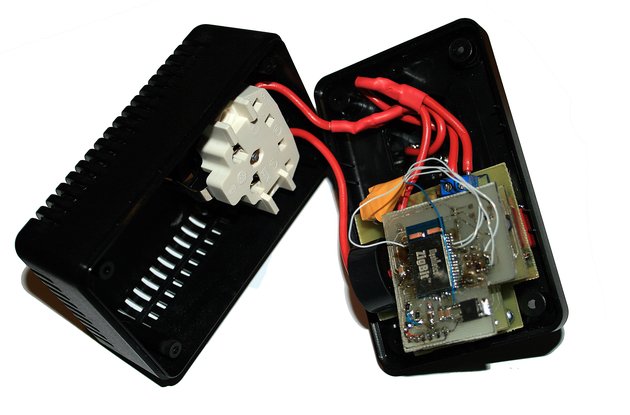
\includegraphics[scale=0.5]{hw_platform/sparrowpower2.png}
\end{center}
\caption{\small \itshape{The Sparrow Power wireless device(inside)}}
\end{figure}